%% Chapter 2: Operating System Foundations
%% Cybersecurity Lab Report — Docker Escape via docker.sock Abuse and Command Injection

\chapter{Operating System Foundations}

%% ─────────────────────────────────────────────────────────────────────────────
\section{The Linux Kernel and Its Role}
%% ─────────────────────────────────────────────────────────────────────────────

The Linux kernel is the single arbitrator of all hardware and process access on a
system. Every container, every process, and every privileged daemon ultimately
operates at the kernel's discretion. Understanding the kernel's design is therefore
a prerequisite for understanding why container isolation is possible, why it is
imperfect, and why the attack described in later chapters succeeds.

Linux follows a \textit{monolithic kernel} architecture: all core subsystems---memory
management, the filesystem layer, the network stack, and the process scheduler---run
in \textit{kernel space} (CPU ring 0). Code executing in ring 0 has unrestricted
access to physical hardware and all kernel data structures. User processes, by
contrast, run in \textit{ring 3} and cannot directly address hardware. Any operation
that requires kernel involvement---reading a file, creating a socket, spawning a
child process---must cross the kernel--user boundary via a \textit{system call}.

\begin{figure}[H]
\centering
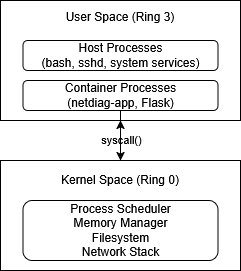
\includegraphics[width=0.4\textwidth]{images/ch2/linux_privilege_rings.png}
% Diagram: Linux Privilege Rings / Kernel--User Space Boundary
% Shows Ring 0 (kernel), Ring 3 (userland), syscall crossing point,
% container processes sitting in ring 3 alongside host processes
\caption{Linux Privilege Rings and the Kernel--User Space Boundary}
\end{figure}

Two privilege domains therefore govern all execution on a Linux host:

\begin{itemize}
    \item \textbf{Kernel space (ring 0):} Executes with full hardware privileges.
          Hosts all subsystems, device drivers, and the syscall dispatch table.
    \item \textbf{User space (ring 3):} Executes without direct hardware access.
          All processes---including container processes---run here.
\end{itemize}

A critically important consequence follows from this design: the Linux kernel has no
native concept of a \textit{container}. The kernel sees only processes, namespaces,
and control groups. All containers running on a host share the \textit{same kernel}.
This shared kernel is the fundamental attack surface exploited throughout this
project. A container process and a native host process are, from the kernel's
perspective, architecturally identical objects differentiated only by their namespace
membership and cgroup assignment.


%% ─────────────────────────────────────────────────────────────────────────────
\section{System Calls --- The Kernel Interface}
%% ─────────────────────────────────────────────────────────────────────────────

System calls (syscalls) are the only sanctioned mechanism by which user-space code
may request privileged kernel services. When a process in ring 3 needs to perform an
operation that requires kernel involvement, it executes a \texttt{syscall} instruction
(or the legacy \texttt{int 0x80} on 32-bit systems). The CPU immediately switches
execution to ring 0, transfers control to the kernel's syscall dispatcher, which
identifies the requested service by number and invokes the appropriate handler. On
completion, the CPU returns to ring 3 and execution resumes in user space.

Each syscall is identified by a unique integer. On x86\_64 Linux, some relevant
numbers include \texttt{clone} (56), \texttt{mount} (165), and \texttt{socket} (41).
The syscall table itself lives in kernel memory and cannot be modified by unprivileged
processes without a kernel exploit.

\begin{figure}[h]
\centering
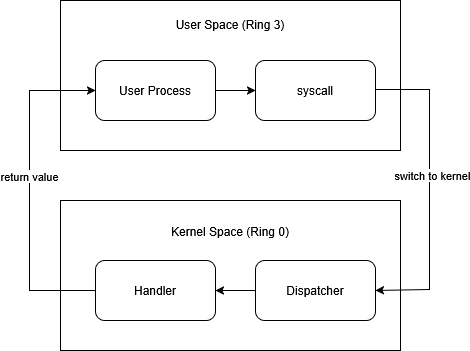
\includegraphics[width=0.8\textwidth]{images/ch2/syscall_flow.png}
% Diagram: Syscall Flow --- User Space to Kernel and Back
% Shows: user process → syscall instruction → kernel dispatch table → handler → return value
\caption{Syscall Flow: User Space to Kernel and Back}
\end{figure}

Several syscalls are directly relevant to container creation and, consequently, to the
attack surface examined in this report:

\begin{itemize}
    \item \texttt{clone(CLONE\_NEWPID | CLONE\_NEWNS | ...)} --- namespace creation;
          this is the syscall that actually instantiates a container's isolated view.
    \item \texttt{unshare()} --- detaches the calling process from one or more of its
          current namespaces.
    \item \texttt{setns()} --- joins an existing namespace identified by a file
          descriptor; the mechanism by which namespace escape is accomplished.
    \item \texttt{execve()} --- replaces the calling process image with a new program.
    \item \texttt{socket(AF\_UNIX, ...)} --- creates a Unix domain socket, the
          underlying transport for \texttt{docker.sock} communication.
\end{itemize}

The following command illustrates syscall observation during container creation:

\begin{lstlisting}[language=bash]
strace -e trace=clone,unshare,mount docker run --rm alpine sh
# shows exact syscalls docker uses to create a container
\end{lstlisting}

Because seccomp operates as a BPF filter interposed at this layer, restricting
syscalls is the primary kernel-level defence against container escapes. Its
limitations in the context of \texttt{docker.sock} abuse are discussed in
Section~\ref{sec:seccomp}.


%% ─────────────────────────────────────────────────────────────────────────────
\section{Process Isolation and the Process Table}
%% ─────────────────────────────────────────────────────────────────────────────

The kernel maintains a single, global process table. Every process on the system---
whether a native host service or a containerised workload---occupies an entry in this
table, represented internally by a \texttt{task\_struct}. The \texttt{task\_struct}
holds all per-process metadata: the process identifier (PID), associated UID/GID,
open file descriptor table, memory map, capability sets, and, critically, a pointer
to the process's \texttt{nsproxy}---the structure linking it to its namespace set.

The apparent isolation of container processes is therefore a \textit{visibility}
property, not a \textit{separation} property. From the host:

\begin{lstlisting}[language=bash]
# On host -- see container process with its real host PID
ps aux | grep flask
\end{lstlisting}

The same Flask process that appears as PID 1 inside its container is visible on the
host with a higher, real PID (e.g., 3847). From inside the container, the process
appears isolated:

\begin{lstlisting}[language=bash]
# From inside the container -- sees only its own namespace PIDs
ps aux
\end{lstlisting}

Key implications for security are as follows. The container's \texttt{init} (PID 1
within the container) is just another process on the host. If cgroup PID limits are
absent, a fork bomb inside a container directly burdens the host's process scheduler.
Parent-child process relationships cross the container boundary in the kernel's view,
even though they are invisible from within the container's PID namespace.


%% ─────────────────────────────────────────────────────────────────────────────
\section{Linux Namespaces --- The Core of Container Isolation}
\label{sec:namespaces}
%% ─────────────────────────────────────────────────────────────────────────────

Linux namespaces partition global kernel resources so that each container receives an
isolated \textit{view} of those resources. Eight namespace types exist in modern
kernels; six are relevant here: PID, NET, MNT, UTS, IPC, and USER. Namespaces are
created via \texttt{clone()} flags or the \texttt{unshare()} syscall, and are
hierarchical---a child process inherits the parent's namespace set unless one or more
\texttt{CLONE\_NEW*} flags override this.

\begin{lstlisting}[language=bash]
ls -la /proc/self/ns/
# lrwxrwxrwx ... pid -> pid:[4026531836]
# lrwxrwxrwx ... net -> net:[4026531992]
\end{lstlisting}

The inode numbers exposed by these symlinks uniquely identify namespace instances.
Two processes sharing the same inode for \texttt{/proc/\textless{}pid\textgreater{}/ns/pid}
are members of the same PID namespace---a fact exploited by detection scripts later
in this report.

\begin{figure}[h]
\centering
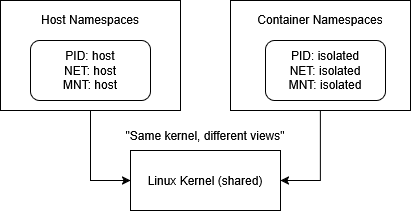
\includegraphics[width=0.8\textwidth]{images/ch2/linux_namespace_hierarchy.png}
% Diagram: Linux Namespace Hierarchy --- Host vs Container View
% Shows host namespace set vs container namespace set;
% shared kernel underneath; PID/NET/MNT split
\caption{Linux Namespace Hierarchy: Host vs Container View}
\end{figure}

The central security implication is concisely stated: namespaces constrain
\textit{what a process sees}, not \textit{what the kernel permits it to do}. A
process that gains access to a privileged communication channel---such as the Docker
daemon socket---can instruct the daemon to perform operations on its behalf that
bypass all namespace restrictions.

%% ── 2.4.1 ─────────────────────────────────────────────────────────────────
\subsection{PID Namespace}
%% ──────────────────────────────────────────────────────────────────────────

The PID namespace gives a container its own process identifier number space, starting
at PID 1. The host kernel maintains the real, globally unique PIDs; the container's
PID namespace provides a translated view. The same process therefore has two PIDs:
its real host PID (e.g., 3847) and its container-local PID (e.g., 1).

PID namespaces are nested: the host PID namespace is the root; each container's PID
namespace is a child. If PID 1 within a container is killed, the kernel delivers
\texttt{SIGKILL} to all remaining processes in that namespace, terminating the
container. Escaping to the host namespace reveals the real PIDs of all container
processes, enabling targeted signal delivery and \texttt{/proc} introspection against
previously opaque workloads.

%% ── 2.4.2 ─────────────────────────────────────────────────────────────────
\subsection{Network Namespace}
%% ──────────────────────────────────────────────────────────────────────────

Each container's network namespace provides an isolated network stack: its own
loopback and Ethernet interfaces, routing table, iptables rule set, and socket table.
The container is connected to the host via a \textit{virtual Ethernet pair}
(\texttt{veth}): one end appears inside the container as \texttt{eth0}; the other end
is attached to the \texttt{docker0} bridge on the host (default subnet
\texttt{172.17.0.0/16}).

Port forwarding (e.g., \texttt{-p 5000:5000}) is implemented as a host-side
iptables DNAT rule that rewrites the destination address of inbound packets to the
container's internal IP. A reverse shell initiated from within the container
traverses this path in reverse: container network namespace $\rightarrow$ \texttt{veth}
pair $\rightarrow$ \texttt{docker0} bridge $\rightarrow$ host NIC $\rightarrow$
attacker.

\begin{lstlisting}[language=bash]
ip netns list                       # list network namespaces
ip link show                        # host: docker0 + veth pairs
docker exec netdiag-app ip addr     # container: only eth0
\end{lstlisting}

%% ── 2.4.3 ─────────────────────────────────────────────────────────────────
\subsection{Mount Namespace}
\label{sec:mountns}
%% ──────────────────────────────────────────────────────────────────────────

The mount namespace isolates the filesystem mount table, giving each container its
own root (\texttt{/}). Docker implements the container's root filesystem using
\textbf{OverlayFS}: read-only image layers (\texttt{lowerdir}) are stacked beneath a
per-container writable layer (\texttt{upperdir}) and merged into a unified view
mounted at the container root.

\begin{figure}[h]
\centering
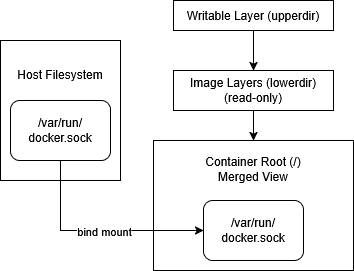
\includegraphics[width=0.6\textwidth]{images/ch2/overlayfs_and_bind_mount.png}
% Diagram: OverlayFS + Bind Mount --- How docker.sock Pierces Namespace Isolation
% Shows: image layers (lower), writable layer (upper), merged view,
% bind mount path from host into container
\caption{OverlayFS and Bind Mount: How \texttt{docker.sock} Pierces Mount Namespace Isolation}
\end{figure}

\textit{Bind mounts} pierce the mount namespace by mapping a host path directly into
the container's mount table. The configuration:

\begin{lstlisting}[language=bash]
-v /var/run/docker.sock:/var/run/docker.sock
\end{lstlisting}

causes the host socket inode to appear simultaneously in both the host and container
mount namespaces. The mount namespace boundary is intact for all other paths, but
\textit{bypassed} for this specific path. This misconfiguration is the root cause of
the escape demonstrated in Chapter~4. Mount namespace membership can be inspected
from inside the container:

\begin{lstlisting}[language=bash]
cat /proc/self/mounts          # shows bind mounts visible in current namespace
findmnt                        # tree view of all mounts
\end{lstlisting}

%% ── 2.4.4 ─────────────────────────────────────────────────────────────────
\subsection{UTS Namespace}
%% ──────────────────────────────────────────────────────────────────────────

The UTS (UNIX Time-sharing System) namespace isolates the system hostname and NIS
domain name. A container may be assigned its own hostname via the \texttt{--hostname}
flag without affecting the host's identity. This namespace has minimal direct
relevance to the attack described in this report and is included for completeness of
the isolation model.

%% ── 2.4.5 ─────────────────────────────────────────────────────────────────
\subsection{IPC Namespace}
%% ──────────────────────────────────────────────────────────────────────────

The IPC namespace isolates System V inter-process communication objects (message
queues, semaphores, and shared memory segments) and POSIX message queues. By default,
container processes cannot access host IPC objects. The flag \texttt{--ipc=host}
removes this isolation, collapsing the container's IPC namespace into the host's.
This configuration is occasionally encountered in high-performance computing
deployments but is not exploited directly in this project.

%% ── 2.4.6 ─────────────────────────────────────────────────────────────────
\subsection{User Namespace}
%% ──────────────────────────────────────────────────────────────────────────

The user namespace maps UIDs and GIDs inside the container to different UIDs and GIDs
on the host. Rootless Docker uses this mechanism: UID 0 inside the container maps to
an unprivileged UID (e.g., 100000) on the host, confining the blast radius of a
container escape.

Standard Docker, however, runs a root-owned daemon and does not enable user namespace
remapping by default. In this configuration, UID 0 inside the container corresponds
to UID 0 on the host for all kernel-mediated operations. The container used in this
project runs as root without user namespace remapping, which can be confirmed from
inside the container:

\begin{lstlisting}[language=bash]
cat /proc/self/uid_map
# "0  0  4294967295" = no remapping; the process is true root
\end{lstlisting}

This absence of remapping is directly relevant to the escape in Chapter~6: filesystem
objects created by the escaped container process are owned by host root, and the
privileged container spawned via \texttt{docker.sock} also runs as host root.


%% ─────────────────────────────────────────────────────────────────────────────
\section{Control Groups (cgroups) --- Resource Enforcement}
%% ─────────────────────────────────────────────────────────────────────────────

Control groups (cgroups) limit, account for, and isolate the resource consumption
of process groups. Docker creates one cgroup per container under
\texttt{/sys/fs/cgroup/}. Two versions of the cgroup interface exist: cgroups v1,
which organises subsystems into separate per-resource hierarchies, and cgroups v2,
which unifies all subsystems under a single hierarchy.

\begin{figure}[h]
\centering
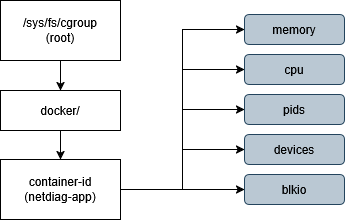
\includegraphics[width=0.6\textwidth]{images/ch2/cgroup_hierarchy.png}
% Diagram: cgroup Hierarchy --- Host vs Container Resource Slice
% Shows: host cgroup root → docker/ slice → per-container cgroup;
% subsystems hanging off each node
\caption{cgroup Hierarchy: Host vs Container Resource Slice}
\end{figure}

Relevant subsystems include:

\begin{itemize}
    \item \texttt{memory} --- limits resident set size; prevents a container from
          exhausting host RAM and triggering the OOM killer against host processes.
    \item \texttt{cpu} --- enforces CPU scheduling quotas.
    \item \texttt{pids} --- caps the number of processes; prevents fork bomb
          propagation to the host scheduler.
    \item \texttt{devices} --- controls access to device nodes; this is the subsystem
          disabled by \texttt{--privileged}.
    \item \texttt{blkio} --- limits block I/O bandwidth.
\end{itemize}

\begin{lstlisting}[language=bash]
# View memory usage for a running container
cat /sys/fs/cgroup/memory/docker/<container-id>/memory.usage_in_bytes

# Inspect cgroup parent via Docker API
docker inspect netdiag-app | grep CgroupParent
\end{lstlisting}

A critical limitation must be stated clearly: \textbf{cgroups enforce resource
boundaries; they do not provide security isolation}. They cannot prevent a process
from abusing a privileged socket, from calling \texttt{setns()} to join another
namespace (given the appropriate capabilities), or from performing any other
privilege-escalation technique. The \texttt{--privileged} flag disables the
\texttt{devices} cgroup subsystem entirely, granting the container access to all host
device nodes.


%% ─────────────────────────────────────────────────────────────────────────────
\section{Capabilities --- Fine-Grained Privilege Model}
\label{sec:capabilities}
%% ─────────────────────────────────────────────────────────────────────────────

Traditional UNIX privilege is binary: a process is either root (all privileges) or
unprivileged (none). Linux capabilities decompose root's monolithic privilege into
approximately forty discrete units, each controlling a distinct class of operations.
This allows Docker to run a container as UID 0 while withholding the most dangerous
kernel permissions.

Each process maintains five capability sets: \texttt{Permitted}, \texttt{Effective},
\texttt{Inheritable}, \texttt{Bounding}, and \texttt{Ambient}. The \texttt{Effective}
set determines what the process may do at any given moment; the \texttt{Bounding} set
acts as a ceiling that no child process may exceed.

Docker's \textbf{default capability set} (retained in containers) includes:
\texttt{CHOWN}, \texttt{DAC\_OVERRIDE}, \texttt{FOWNER}, \texttt{KILL},
\texttt{NET\_BIND\_SERVICE}, \texttt{SETUID}, \texttt{SETGID}, \texttt{SYS\_CHROOT},
\texttt{AUDIT\_WRITE}, \texttt{MKNOD}, \texttt{NET\_RAW}, \texttt{SETFCAP}, and
\texttt{SETPCAP}.

Docker \textbf{drops by default}: \texttt{SYS\_ADMIN}, \texttt{NET\_ADMIN},
\texttt{SYS\_PTRACE}, \texttt{SYS\_MODULE}, and others. Of these,
\texttt{CAP\_SYS\_ADMIN} deserves special attention: it is functionally near-
equivalent to root, enabling \texttt{mount()} calls, namespace manipulation via
\texttt{setns()} and \texttt{unshare()}, and a wide range of other privileged
operations.

\begin{lstlisting}[language=bash]
# Inspect capability sets from inside the container
capsh --print
# or directly from procfs
cat /proc/self/status | grep Cap
capsh --decode=<hex_value>
\end{lstlisting}

The container used in this project runs as root with Docker's default capability set
and \textit{without} \texttt{--privileged}. This means direct kernel escape via
\texttt{CAP\_SYS\_ADMIN} is not available. However, the \texttt{docker.sock} escape
entirely circumvents the capability model: the attacker does not perform privileged
syscalls from inside the container; instead, they instruct the Docker \textit{daemon}
to spawn a new privileged container on their behalf. The daemon executes with full
host root privileges and is unaffected by the attacking container's capability
restrictions. This is detailed in Chapter~6.


%% ─────────────────────────────────────────────────────────────────────────────
\section{Seccomp --- Syscall Filtering}
\label{sec:seccomp}
%% ─────────────────────────────────────────────────────────────────────────────

Seccomp (Secure Computing Mode) restricts the set of syscalls available to a process.
Docker applies a default seccomp profile that blocks approximately 44 syscalls
considered dangerous or unnecessary for typical container workloads. It represents the
last kernel-level line of defence between a container process and the host kernel.

Seccomp operates by attaching a BPF (Berkeley Packet Filter) program to the target
process. Every syscall invocation is evaluated against this program before the kernel
handler executes. Docker uses \texttt{SECCOMP\_MODE\_FILTER}, which allows a
fine-grained BPF rule set rather than the minimal
\texttt{SECCOMP\_MODE\_STRICT} (which permits only \texttt{read},
\texttt{write}, \texttt{exit}, and \texttt{sigreturn}).

Docker's default seccomp profile blocks, among others: \texttt{kexec\_load},
\texttt{ptrace}, \texttt{reboot}, \texttt{init\_module}, and
\texttt{perf\_event\_open}. The \texttt{mount} syscall is also blocked, preventing a
container process from directly mounting host filesystems.

Critically, the default profile \textbf{does not block} Unix domain socket
operations. The \texttt{socket(AF\_UNIX, ...)} syscall and all subsequent socket I/O
syscalls used to communicate with \texttt{docker.sock} are fully permitted. The
escape described in this report does not require bypassing seccomp.

\begin{lstlisting}[language=bash]
# Confirm seccomp profile for the running container
docker inspect netdiag-app | grep Seccomp

# Inspect blocked syscalls from the default profile
cat /etc/docker/seccomp.json | python3 -m json.tool | grep '"name"' | head -20
\end{lstlisting}

The flags \texttt{--security-opt seccomp=unconfined} and \texttt{--privileged} both
disable seccomp filtering entirely, significantly widening the attack surface.


%% ─────────────────────────────────────────────────────────────────────────────
\section{AppArmor and Linux Security Modules}
%% ─────────────────────────────────────────────────────────────────────────────

Linux Security Modules (LSMs) extend the kernel's Discretionary Access Control (DAC)
model with Mandatory Access Control (MAC). Where DAC enforces access rules based on
object ownership and permission bits, MAC enforces rules defined by a security policy
that neither the object owner nor even root can override within the kernel. LSM hooks
are inserted at kernel object boundaries---files, sockets, IPC objects---and are
invoked before every access decision.

AppArmor is the LSM shipped as Docker's default on Debian, Ubuntu, and Kali Linux.
It is a \textit{path-based} MAC system: profiles specify which filesystem paths a
process may access, which capabilities it may exercise, and what network operations
are permitted.

Docker loads its \texttt{docker-default} AppArmor profile for every container unless
overridden with \texttt{--security-opt apparmor=unconfined}. This profile restricts
access to sensitive \texttt{/proc} and \texttt{/sys} paths, and redundantly denies
the \texttt{mount} syscall. However, the \texttt{docker-default} profile does not
explicitly deny access to Unix domain sockets. Communication with
\texttt{docker.sock} is therefore \textit{permitted} by AppArmor as well as by
seccomp.

\begin{lstlisting}[language=bash]
# Confirm AppArmor profile assigned to the container
docker inspect netdiag-app | grep AppArmor

# List all loaded profiles on the host
aa-status
\end{lstlisting}

Falco, the runtime intrusion detection system evaluated in Chapter~11, operates at a
comparable layer via \texttt{fanotify} and eBPF probes rather than AppArmor profiles,
giving it visibility into \texttt{docker.sock} accesses that AppArmor silently permits.


%% ─────────────────────────────────────────────────────────────────────────────
\section{The \texttt{/proc} Filesystem}
%% ─────────────────────────────────────────────────────────────────────────────

\texttt{/proc} is a virtual filesystem generated entirely in kernel memory; no data
is stored on disk. It exposes kernel data structures as a navigable file hierarchy,
providing the primary introspection interface for process monitoring, namespace
inspection, and container detection tooling.

Each running process is represented by a directory \texttt{/proc/\textless{}pid\textgreater{}/}
containing, among others:

\begin{itemize}
    \item \texttt{ns/} --- symbolic links to namespace membership; inode comparison
          reveals whether two processes share a namespace.
    \item \texttt{fd/} --- symbolic links to all open file descriptors; reveals open
          sockets and files.
    \item \texttt{maps} --- the process memory map.
    \item \texttt{status} --- capability hex values, real and effective UIDs, and
          other per-process metadata.
    \item \texttt{mounts} --- the mount table as seen from this process's mount
          namespace; shows bind mounts including \texttt{docker.sock}.
    \item \texttt{cmdline} --- the command used to invoke the process.
\end{itemize}

The symlink \texttt{/proc/self} always resolves to the calling process's own
\texttt{/proc} directory. \texttt{/proc/net/unix} lists all Unix domain sockets
open on the system, confirming \texttt{docker.sock} availability.

\begin{lstlisting}[language=bash]
# From inside the container
ls -la /proc/self/ns/
cat /proc/self/mounts | grep docker
cat /proc/self/status | grep -E "Uid|Cap"

# From the host -- compare namespace inodes
readlink /proc/1/ns/mnt                # host init
readlink /proc/<container-pid>/ns/mnt  # container process
\end{lstlisting}

If the two \texttt{mnt} namespace inodes differ, the processes reside in separate
mount namespaces---confirming the container boundary. If they match after an escape
attempt, the escape succeeded and the attacker's process has joined the host mount
namespace. The detection script \texttt{detect.sh} relies on \texttt{lsof}, which
internally reads \texttt{/proc/*/fd/} to identify open socket descriptors.


%% ─────────────────────────────────────────────────────────────────────────────
\section{How the Kernel Sees a Container vs a Process}
\label{sec:kernel-synthesis}
%% ─────────────────────────────────────────────────────────────────────────────

The preceding sections can now be synthesised into a unified model. From the kernel's
perspective, a container is not a discrete entity; it has no dedicated data type
and no privileged representation. A container is simply a process tree whose members
share a common namespace set, are enrolled in a common cgroup hierarchy, hold a
specific capability set, and are subject to an optional seccomp filter and AppArmor
profile.

Internally, each process is represented by a \texttt{task\_struct}. The fields
relevant to container isolation are:

\begin{itemize}
    \item \texttt{nsproxy} --- pointer to the \texttt{nsproxy} structure holding
          references to the process's PID, NET, MNT, UTS, IPC, and USER namespace
          instances.
    \item \texttt{cgroups} --- pointer to the process's cgroup membership.
    \item Capability bitmasks (\texttt{cap\_permitted}, \texttt{cap\_effective}, etc.).
    \item Pointer to the attached seccomp BPF filter (if any).
\end{itemize}

\begin{figure}[h]
\centering
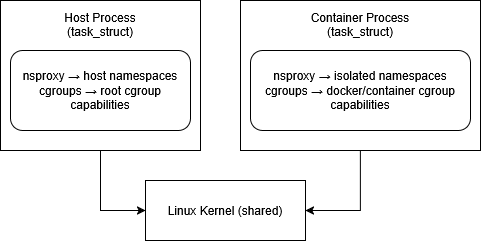
\includegraphics[width=0.9\textwidth]{images/ch2/kernel_view.png}
% Diagram: Kernel View --- Host Process vs Container Process (task\_struct comparison)
% Shows: two task\_struct boxes side by side; host process with host nsproxy;
% container process with its own nsproxy pointing to new NS objects;
% both pointing to same kernel, same cgroup root
\caption{Kernel View: Host Process vs Container Process (\texttt{task\_struct} comparison)}
\end{figure}

All containers on a host share:

\begin{itemize}
    \item The kernel binary and all loaded kernel modules.
    \item The kernel's physical memory (mapped, not directly accessible, but subject
          to shared-kernel vulnerabilities).
    \item The kernel's syscall dispatch table.
    \item The \texttt{/proc} filesystem (filtered per PID namespace).
\end{itemize}

A process holding \texttt{CAP\_SYS\_ADMIN} may call \texttt{setns()} to join any
namespace for which it possesses a valid file descriptor---this is the mechanism
underlying direct namespace escape techniques. The \texttt{docker.sock} escape used
in this project is architecturally different: the attacker process does not require
\texttt{CAP\_SYS\_ADMIN} and does not call \texttt{setns()} directly. Instead, it
communicates with the Docker daemon over the Unix socket. The daemon---which runs as
root on the host with an unrestricted capability set---performs all privileged
operations on the attacker's behalf. The kernel enforces nothing about the daemon's
own operations; it is a fully trusted root process.

Table~\ref{tab:isolation-gaps} summarises the isolation stack and its limitations as
they apply to the attack:

\begin{table}[h]
\centering
\caption{Container Isolation Stack: Mechanisms and Gaps}
\label{tab:isolation-gaps}
\begin{tabular}{|l|l|l|}
\hline
\textbf{Mechanism} & \textbf{What It Isolates} & \textbf{What It Does Not Stop} \\
\hline
Namespaces  & Resource visibility               & Shared kernel; daemon API access \\
cgroups     & Resource consumption              & Privilege escalation             \\
Capabilities & Privilege scope                 & Socket-based API access          \\
Seccomp     & Syscall surface                   & \texttt{AF\_UNIX} socket comms   \\
AppArmor    & File and capability access        & \texttt{docker.sock} by default  \\
\hline
\end{tabular}
\end{table}

The table illustrates why the \texttt{docker.sock} escape is particularly robust: it
does not conflict with any single layer of the isolation stack. No namespace prevents
it, no cgroup limits it, no capability check blocks it, seccomp permits the
underlying socket syscalls, and AppArmor's default profile allows Unix socket access.
Chapter~8 returns to this table to explain, in attack-flow terms, why each layer
fails to interrupt the exploit chain.